\documentclass[]{beamer}
\usepackage[T1]{fontenc}
\usepackage{lmodern}
\usepackage[francais]{babel}
\usepackage[utf8]{inputenc}
\usepackage{amsmath}
\usepackage{amsfonts}
\usepackage{amssymb}
\usepackage{url}
\usepackage{calc}
\usefonttheme[onlymath]{serif}

\author{Pierre \textsc{Bienaimé}\\Bastien \textsc{Bonnet}\\Mathieu \textsc{Chataigner}\\Mathieu \textsc{Fresquet}\\Pâris \textsc{Meuleman}\\Yves \textsc{Parès}\\Thibaut \textsc{Reiter}}
\title{Projet Informatique répartie 2010 :\\BlatteWar}
\institute{INSA de Rouen, ASI}

\usepackage{insaBeamer}

\begin{document}

\addtocounter{section}{-1}
\section*{Page de garde}

\begin{frame}
  \pageDeGarde{\insertauthor}{\inserttitle}{}
\end{frame}

\begin{frame}
  % Présentation du plan générale
  \thispagestyle{empty}
  \begin{picture}(0,0)
    \put(-99.5,-20){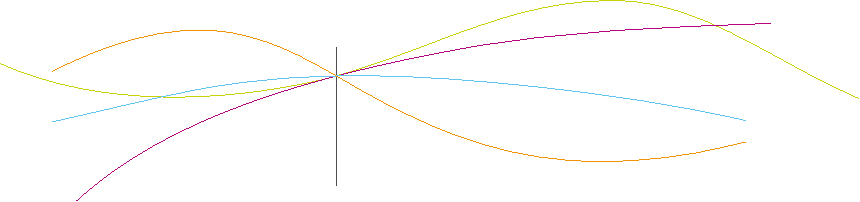
\includegraphics[width=18cm,height=3.5cm]{images/vol3.pdf}}
    \put(100.5,-130){\begin{turn}{90} {\color{GRIS}\rule{70mm}{1pt}} \end{turn}}
%    \inserttocsectionnumber
    \put(110,-30){\begin{minipage}{8cm}\tableofcontents[hideallsubsections]
 \end{minipage}}
  \end{picture}
\end{frame}

\section{Présentation générale}

\subsection{Le sujet}

\begin{frame}[c]{\insertsubsection{}}
    \begin{block}{Sujet}
    LabyrintheBattle, adaption d'un Robot Battle, devenu Blatte War.
    \end{block}

    \begin{block}{Le jeu}
        \begin{itemize}
        \item Un labyrinthe arène, 
        \item Les clients viennent tester leur IA,
        \item Les joueurs incarnent une blatte.
        \end{itemize}
    \end{block}
\end{frame}


\section{Cahier des charges}

\subsection{Architecture de l'application}
\begin{frame}[c]{\insertsubsection{}}
    \begin{block}{Fonctionnalités :}
        \begin{itemize}
        \item Une interface permettant aux utilisateurs d'implémenter leur IA \pause
        \item Un serveur qui gère :
        
            $\bullet$ Les connections des clients
            
            $\bullet$ Le match (arène et interactions des blattes)
            
            $\bullet$ Le déroulement de la partie (phases)
        \end{itemize}
    \end{block}
\end{frame}

\subsection{Le jeu}
\begin{frame}[c]{\insertsubsection{}}
        \begin{block}{Règles du jeu}
        \begin{itemize}
        \item Tour par tour
        \item Nombre défini de points de vie
        \item 3 actions possibles : Attaque, Déplacement ou Attente
        \item Condition de victoire : survie ou case sortie
        \end{itemize}
    \end{block}
\end{frame}


\begin{frame}[c]{}
    \begin{block}{L'arène}
        \begin{itemize}
        \item Constituées de cases, Sol ou Mur
        \item Une ou plusieurs cases sortie
        \item Chaque case possède 0 ou 1 propriété
        \end{itemize}
    \end{block}
    
    \pause
    
    \begin{block}{Les blattes}
        \begin{itemize}
        \item 1 blatte par client
        \item Possèdent un champ de vision de portée 1 case
        \item Peuvent se déplacer d'une case maximum par tour
        \end{itemize}
    \end{block}
\end{frame}

\section{Conception}

\subsection{Diagramme de classe}

\begin{frame}[c]{\insertsubsection{}}
    \begin{block}
        Communication par 2 Remote Objects :
        \begin{description}
            \item[Serveur] Classe Simulateur
            \item[Client] Interface Joueur: \\
                méthode determinerAction(Blatte, ChampVision) : Action
        \end{description}

        Action = Attente OU Deplacement OU Attaque
    \end{block}
\end{frame}

\begin{frame}
    \begin{block}
        Architecture du jeu :
        \begin{itemize}
            \item MoteurJeu
            \item Arene > Case > Blatte
            \item Case = Mur OU Sol OU Depart OU Sortie
            \item Singleton DescPropriete: \\
                 méthode effet(Blatte)
             \item Propriete
        \end{itemize}
    \end{block}
\end{frame}

\subsection{Choix des technologies}

\begin{frame}[c]{\insertsubsection}
    \begin{block}{Technologies utilisées :}
        \begin{itemize}
        \item Communication : RMI 
        \item Serveur : EJB
        \item Affichage : JSP
        \item Rapports de match : XML et XSLT
        \end{itemize}
    \end{block}
\end{frame}



\section{Développement}

\subsection{Démonstration}

\begin{frame}[c]{\insertsubsection{}}
    \begin{center}
    	\huge{Démonstration} 
     \end{center}
\end{frame}




\section{Conclusion}

\subsection{Respect du cahier des charges}

\begin{frame}[c]{\insertsubsection{}}
    \begin{block}{Objectifs atteints}
        \begin{itemize}
        \item Cahier des charges réaliste dès le départ
        \item Cahier des charges  complétement respecté
        \end{itemize}
    \end{block}
        \begin{block}{Élements supplémentaires}
        \begin{itemize}
        \item Un rapport XML
        \end{itemize}
    \end{block}
\end{frame}

\subsection{Difficultés rencontrées}

\begin{frame}[c]{\insertsubsection}
    \begin{block}{Difficultés rencontrées}
        \begin{itemize}
        \item La communication RMI
        \item Les callbacks
        \item Les erreurs Jboss.
        \end{itemize}
    \end{block}
\end{frame}

\subsection{Perspectives}

\begin{frame}[c]{\insertsubsection}
    \begin{block}{Perspectives}
        \begin{itemize}
        \item Changer le champ de vision
        \item Améliorer les IA, pouvoirs, objets, ...
        \item Proposer un service d'upload
        \item Proposer des paris sur la victoire
        \item Un mode par équipe
        \item Un mode capture the flag
        \end{itemize}
    \end{block}
\end{frame}


\begin{frame}
  \pageFinale{\insertauthor}
\end{frame}

\end{document}
